\chapter{Methodology}
\label{chap:2}
\ChapterPageStuff{2}

\section{Preamble}

\section{Logging mechanism}\label{Ch2:LoggingMechanism} The logging mechanism will need to meet the requirements discussed in \Cref{sec:EventLogging} to capture the required logs to apply system utilisation analysis on it. \Cref{fig:CH2_SystemA_Arch_Design} is the design for the logging mechanism to capture the user's activities. In this figure, the logging mechanism is split up into two functional requirements parts (\textbf{F/R}) which consist of the client and server functional requirements.\par Each functional requirement has interface requirements with each other to transfer any of the required data or start a process in other functional requirements. These interfaces are labelled as \textbf{I/F} in \Cref{fig:CH2_SystemA_Arch_Design}.

\begin{figure}[!htb] % An h :here, t: top, b: bottom.
	\centering % cent the figure
	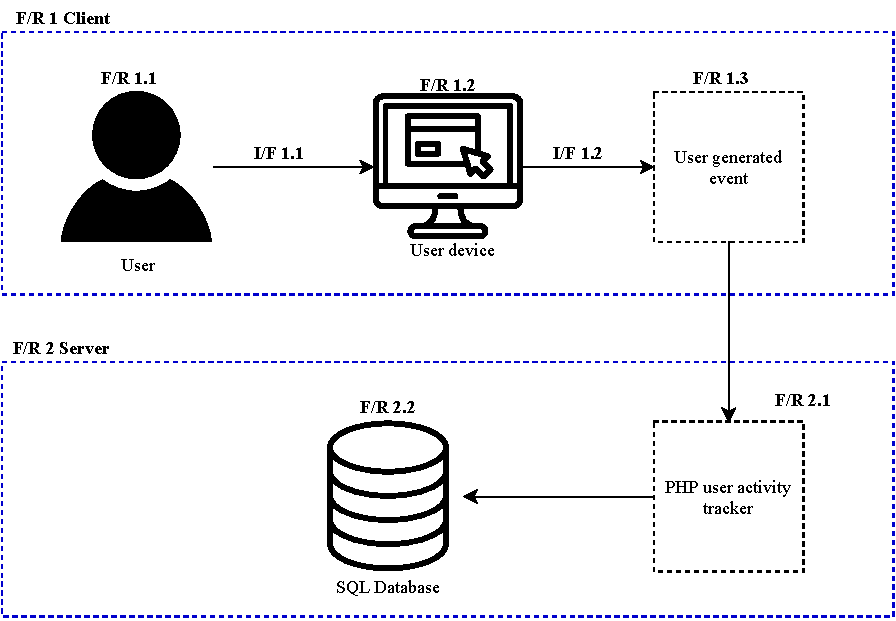
\includegraphics[width=0.9\textwidth]{Chapter2/SystemA_Architecture_Diagram/SystemA_Architecture_Diagram.pdf}
	\caption[System A logging mechanism architecture design]
	{\textit{System A logging mechanism architecture design}}\label{fig:CH2_SystemA_Arch_Design}
\end{figure}

The client's functional requirements (F/R 1) consist of the user interacting with a device on the website. In \Cref{tbl:Ch2_Client_Functional_Requirements} is the functional requirements that are on the client-side of the user activity logging mechanism.

\begin{table}[!htb]
	\centering
	\small
	\caption[Client functional requirements]
	{\textit{Client functional requirements (F/R 1)}}
	\label{tbl:Ch2_Client_Functional_Requirements}
	\begin{tabularx}{\textwidth}{|l|l|X|}
		\hline \textbf{Requirement ID} & \textbf{Name} & \textbf{Description} \\
		\hline F/R 1.1 & User & The user serves as primary initiator of the activity events.\\
		\hline F/R 1.2 & User's device & The device that user uses to access the website from where the activity events are generated.\\
		\hline F/R 1.3 & User generated events & These are any activity events that user started that needs to communicate back to server.\\
		\hline
	\end{tabularx}
\end{table}

The functional requirements in \Cref{tbl:Ch2_Client_Functional_Requirements} needs to interface with each other. These interfaces in \Cref{tbl:Ch2_Client_Interface_Requirements} parses the input from the user to create basic user event log.

\begin{table}[!htb]
	\centering
	\small
	\caption[Client interface requirements]
	{\textit{Client interface requirements for F/R 1}}
	\label{tbl:Ch2_Client_Interface_Requirements}
	\begin{tabularx}{\textwidth}{|l|l|X|}
		\hline \textbf{Requirement ID} & \textbf{Name} & \textbf{Description} \\
		\hline I/F 1.1 & User input & The user starts the activity events by using the user interface to give the website any input.\\
		\hline I/F 1.2 & Log parsing of logging points & The user generated event is captured to get some of the key logging points of \Cref{tbl:CH1_Log_Basic_Attributes}.\\
		\hline
	\end{tabularx}
\end{table}

The server functional requirements in \Cref{tbl:Ch2_Server_Functional_Requirements} captures the rest of the key logging points and complete the event log to be stored in a database. 

\begin{table}[!htb]
	\centering
	\small
	\caption[Server functional requirements]
	{\textit{Server functional requirements (F/R 2)}}
	\label{tbl:Ch2_Server_Functional_Requirements}
	\begin{tabularx}{\textwidth}{|l|l|X|}
		\hline \textbf{Requirement ID} & \textbf{Name} & \textbf{Description} \\
		\hline F/R 2.1 & User activity logger & The rest of the key logging points are captured and the event log is completed to stored in a database.\\
		\hline F/R 2.2 & Database & The event log is stored in a database until it is needed for further analysis.\\
		\hline
	\end{tabularx}
\end{table}

The interfaces in \Cref{tbl:Ch2_Server_Interface_Requirements} for the client functional requirement (F/R 2) is to obtain the base log from client functional requirement (F/R 1) and finally store the completed log into a database.

\begin{table}[!htb]
	\centering
	\small
	\caption[Server interface requirements]
	{\textit{Server interface requirements for F/R 2}}
	\label{tbl:Ch2_Server_Interface_Requirements}
	\begin{tabularx}{\textwidth}{|l|l|X|}
		\hline \textbf{Requirement ID} & \textbf{Name} & \textbf{Description} \\
		\hline I/F 2.1 & Log parsing to server & The captured log is parsed onto the server for further processing of the captured user generated event.\\
		\hline I/F 2.2 & Store in database & The event log is send to a database for storing.\\
		\hline
	\end{tabularx}
\end{table}

\clearpage

\subsection{Logging points}
In \Cref{sec:Ch1_LoggignPoints} the basic log event attributes needs to be identified to capture the needed logging points that will be used to create the event log. Tracking the events can be divided in different events types as in \Cref{tbl:Ch2_User_ActivityTypes}. \par Accessing a certain web page is used in the utilisation analysis to track which part of the website is being visited by the user. Certain session changes have direct input from the user like login in or clicking on a log out button. \par The rest of the user events are any other activities that the user does on the page excluding the previous two types of events in \Cref{tbl:Ch2_User_ActivityTypes}. These events can be further divided into other types for the system utilisation analysis.

\begin{table}[!htb]
	\centering
	\small
	\caption[User activity types]
	{User activity types}
	\label{tbl:Ch2_User_ActivityTypes}
	\begin{tabularx}{\textwidth}{|l|X|}
		\hline \textbf{Activity Type} & \textbf{Description} \\
		\hline Page accessed & The user may enter different web pages in a session. Tracking which pages the user navigates through.\\
		\hline Session changes & This is any user activities that directly involves extension session before their session times out after a period of inactivity. This also tracks when the session starts as any login attempt is a user based activity.\\
		\hline General user events & Any events that is other than accessing a certain web page that user initiates that communicates with the server. Most of the user activities will have this event type.\\ 
		\hline
	\end{tabularx}
\end{table}

\begin{table}[!htb]
	\centering
	\small
	\caption[Key logging points]
	{\textit{Key logging points}}
	\label{tbl:Ch2_KeyLogging_Points}
	\begin{tabularx}{\textwidth}{|l|X|}
		\hline \textbf{Logging point} & \textbf{Description} \\
		\hline Identification number & The activity identification is an incremental number of the event that is logged.\\
		\hline Timestamp & This is the time which the event took place.\\
		\hline Activity type & Each event can be classified into types. \\
		\hline \textbf{UserID} & Each user has a unique identifier which is a numerical identification number that is foreign key reference to the User table. \\
		\hline \textbf{Area} & This information is logged to track user activities per Area that represents different software systems that the user can use. \\
		\hline \textbf{Controller} & Each event will point back to an controller that process the request. \\
		\hline \textbf{GroupID} & This foreign key reference to the Group table is contract groups identification number. \\
		\hline \textbf{MetaData} & The meta data of the event contains request parameters, the HTML element from which the request is initiated and other relevant request data of the event. This can also be other meta data is important to get that adds more information about the user's activity using certain controls on System B as in \Cref{fig:CH2_SystemBMetaData}. \\
		\hline
	\end{tabularx}
\end{table}

\begin{figure}[!htb]
	\centering
	\begin{lstlisting}[style=json] 
		{ "RequestOrigin" : "/Area4/Controller4",
		  "RequestElementID" : "Button4",
		  "RequestParameters": {
		  "Parameter1": 4,
		  "Parameter2": "Hello World!",
			"Parameter3": true
			"Parameter4": 40.404
		  }		
		}
	\end{lstlisting}
	\caption[System B meta data JSON]
	{\textit{System B meta data JSON}}\label{fig:Ch2_Metadata_Json_Example}
\end{figure}

\section{System utilisation analysis}

\section{integration}

\section{Conclusion}